\chapter{CONCLUSIONES\label{sec:conclusiones}}

\clearpage

TODO

\section{Conclusiones técnicas}

\subsection{Beneficios de las pruebas de software}

Las pruebas de software ahorran tiempo y dinero a una organización al reducir los costos de desarrollo y mantenimiento del software. Las pruebas de software crean garantías de estabilidad en el desarrollo de nuevas características.

El tiempo de desarrollo de las nuevas funciones se reduce especificando un conjunto de casos de prueba que la nueva característica debe cumplir para que se considere completa y entregable. Una vez que estos casos de prueba están en su lugar, los costos generales de mantenimiento se reducen.

Hay que tener bien claro los objetivos de las pruebas de software. Si bien es importante probar que los usuarios pueden usar la aplicación correctamente (iniciar sesión, guardar el estado de un objeto, etcétera), es igualmente importante probar que el sistema no se rompe cuando se envían datos incorrectos o se realizan acciones inesperadas.

\subsection{Beneficios de las pruebas de rendimiento}

Los problemas relacionados con el rendimiento en la producción afectan los ingresos que genera la aplicación y también es muy costoso de solucionar. Las pruebas de rendimiento no solo se realizan para medir en general el tiempo de respuesta de la aplicación, sino también para comprender el comportamiento del sistema con otras aplicaciones en el sistema.

Las pruebas de rendimiento, implementadas correctamente y realizadas a lo largo del ciclo de desarrollo, pueden reducir significativamente la cantidad de fallas experimentadas por una aplicación.

La pruebas de rendimiento han servido, entre otras cosas, para:

\begin{itemize}
  \item Demostrar que el sistema cumple con los criterios de rendimiento.
  \item Validar y verificar atributos de la calidad del sistema: escalabilidad, fiabilidad, uso de los recursos, etcétera.
  \item Medir qué partes del sistema o de carga de trabajo provocan que el conjunto rinda peor.
  \item Exponer memory leaks.
  \item Verificar que las políticas de recolección de basura (garbage collection) son adecuadas.
  \item Verificar que las agrupaciones de conexiones se están reciclando.
  \item Verificar que los manejadores de archivos se están reciclando.
\end{itemize}

\subsection{Beneficios de la arquitectura de las aplicaciones web}

El objetivo de separar las distintas funcionalidades en distintos servidores es aumentar la escalabilidad del sistema de cara a obtener un mayor rendimiento. Al separar las distintas funcionales en distintos servidores, cada uno de ellos se puede configurar de forma adecuada a los requisitos que presenta cada uno de ellos.

Por ejemplo, para el servidor web hace falta una máquina con una buena conexión a Internet, rápido pero sin grandes necesidades de almacenamiento. Sin embargo, para el servidor de bases de datos hace falta una máquina con mucha memoria y con un disco duro de alta capacidad de almacenamiento y rápido para mantener todos los datos.

Otra ventaja que se obtiene al separar las funcionalidades, es que al aislar la lógica de negocio y la lógica de datos en servidores separados que no están conectados directamente a Internet se aumenta el nivel de seguridad, ya que no es tan fácil acceder a ellos.

\subsection{Beneficios de las aplicaciones web en tiempo real}

Podemos afirmar que las aplicaciones web en tiempo real son necesarias. La razón principal no es la inmediatez en las interacciones, sino las mejoras en el rendimiento de la aplicación.

Los servidores web, aunque se encargan de gestionar los mensajes de los clientes, se ahorran los DDoS involuntarios por demasiados clientes conectándose a la vez. El tráfico de red disminuye, algo bastante conveniente con las actuales tarifas para móviles, y las aplicaciones sólo consumen CPU cuando es realmente necesario, y no cada periodo de tiempo de forma fija.

Es cierto que el tiempo real es en parte la excusa perfecta para ver hasta dónde puede llegar la tecnología, pero eso no quita que no nos pueda resultar útil. Podemos encontrar muchos ejemplos de aplicaciones que hacen uso de tiempo real y que son bastante útiles.

\subsection{Beneficios de los WebSockets}

Resulta que hay un gran abismo entre implementar el protocolo WebSocket en una aplicación web, y llevar esa implementación a producción. Algunas de las librerías populares podrían matar tu servidor inmediatamente si la cantidad de conexiones aumenta, en otros casos empiezas a notar pérdida de memoria por cada conexión WebSocket que no fue propiamente desconectada.

Los problemas que pueden producirse en producción usando WebSockets debería medirse a través de las pruebas de rendimiento.

Si bien, la implementación en producción de los WebSockets trae consigo enormes problemas, también presenta los mejores beneficios:

\begin{itemize}
  \item Tiempo de respuesta más rápido que otros mecanismos, ideal para chats.
  \item Aplicaciones más rápidas, ya que la comunicación queda permanentemente abierta.
  \item Y modernas, con excelentes herramientas para backend y frontend.
\end{itemize}

\subsection{Beneficios de las aplicaciones web en Node.js}

Cuando Node.js se introdujo en la comunidad tecnológica en 2009 como una herramienta para crear aplicaciones web escalables en el lado del servidor, se presentaron muchos beneficios que incluyen, entre otros, el uso del modelo de entrada/salida no bloqueante dirigido por eventos y la programación asíncrona de un solo hilo.

\begin{figure}[htp!]
  \centering
  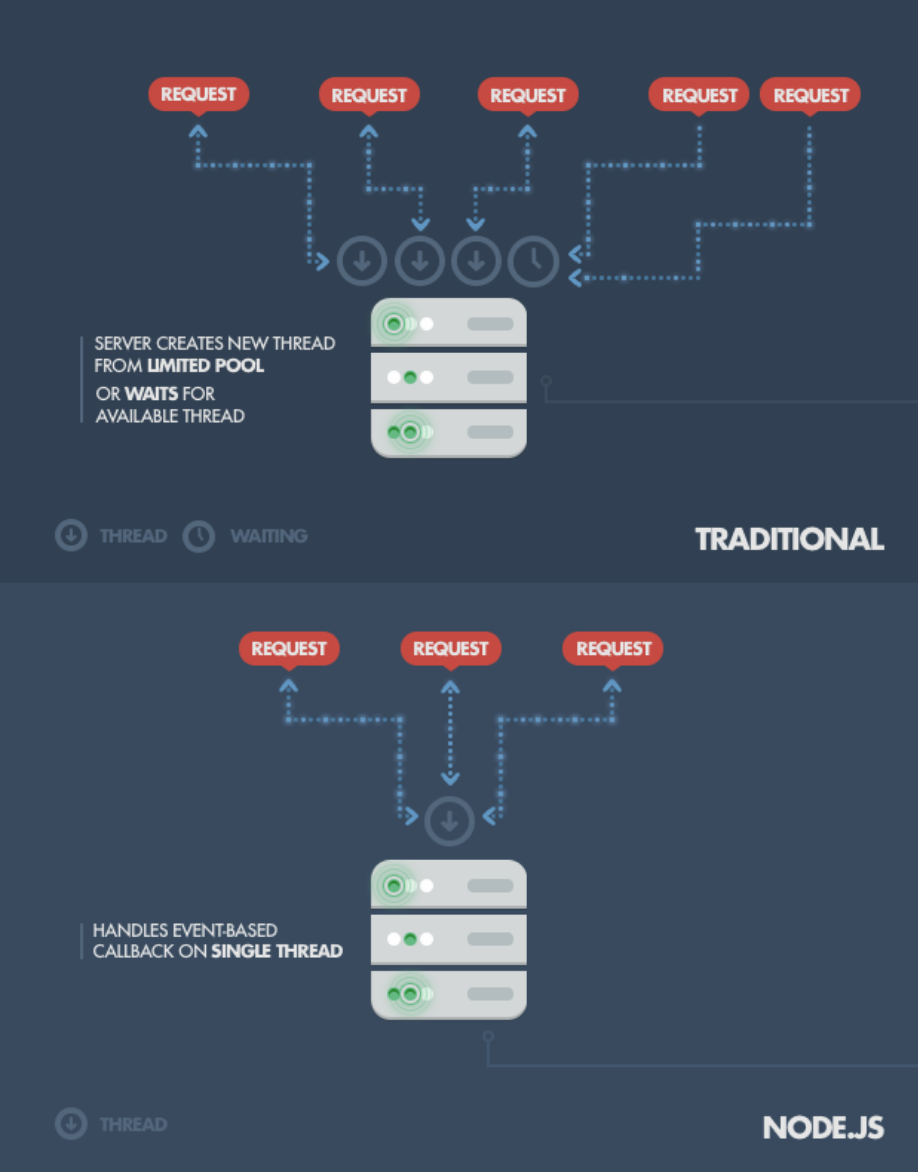
\includegraphics[scale=0.3,clip=true]{nodejs_vs_threadgroup}
  \caption{Thread Group vs Node.js}
  \label{fig:nodejs_vs_threadgroup}
\end{figure}

Node.js te permite escribir el mismo idioma tanto para tu frontend como para tu backend, ahorrandote el estrés de aprender un nuevo idioma para alguna implementación simple y también te ayuda a mantener el mismo patrón de diseño en todo momento.

En este proyecto hemos optado por crear el backend con Node.js, ya que este ofrece más posibilidades y es de más bajo nivel que otros lenguajes. Además, ofrece un rendimiento impecable y como decíamos antes, el proceso de desarrollo es ágil debido a la facilidad de inclusión de paquetes para crear funcionalidad específica mediante npm. Si queremos crear un servicio RESTful con capacidades en tiempo real, la combinación de Express.js con WebSockets nos permite hacerlo de manera fácil y rápida.

\subsection{Memory leaks en Node.js}

La pérdida de memoria es muy común en las aplicaciones de Node.js, especialmente en las de gran escala con tráfico razonable, y muchas empresas grandes la han sufrido.

Una aplicación de Node.js se inicia sólo una vez, no para cada solicitud entrante. Esto hace que el manejo peticiones sea más rápido, ya que solo hace la lógica para cada petición. sin necesidad de trabajo repetitivo, también ahorra los recursos necesarios para este proceso de iniciación.

Pero esto conlleva un precio, que tienes que ocuparse del uso de la memoria de la aplicación, ya que consumirá la memoria continuamente durante su tiempo de ejecución y, si no se maneja el uso de la memoria de manera eficiente, puede agotarse la memoria.

\subsubsection{Causas comunes de memory leak}

Teniendo en cuenta la gestión de memoria en Node.js, podemos definir tres de las causas más comunes de pérdida de memoria que deberíamos tener cuidado al usarlas en un código:

\begin{itemize}
  \item Variables globales. Dado que tienen una ruta directa al nodo raíz, permanecerán en la memoria mientras la aplicación se esté ejecutando, por lo que se debe tener cuidado al configurar las variables globales y la cantidad de datos que se establecerá en ellas.
  \item Referencias múltiples. La configuración de varias referencias al mismo objeto también puede causar problemas, ya que puede eliminar una referencia y olvidar la otra, lo que mantendrá el objeto en cuestión ocupando espacio.
  \item Closures. En los closures, simplemente mantiene las referencias a los objetos que se utilizarán más adelante. esta característica tiene muchas ventajas, pero si se usa sin precaución, puede causar grandes problemas, ya que estas referencias mantendrán a los objetos en la pila y estos pueden ser grandes.
\end{itemize}

\subsubsection{V8 Inspector y Chrome DevTools}

Existen muchas herramientas y bibliotecas que se utilizan para detectar memory leaks en Node.js, todas siguen el mismo concepto para detectar memory leaks de comparar diferentes volcados de pila (heap dump) y verificar los resultados, e intentan forzar la ejecución del garbage collector antes de tomar cualquier head dump para hacer asegurarse de que la pérdida es real.

Una herramienta muy importante, desde mi punto de vista, es el V8 Inspector. Muy útil, especialmente cuando se usa con Chrome DevTools en la fase de desarrollo, ya que te permite monitorear el rendimiento de uso de la memoria para verificar si hay alguna pérdida potencial en el código y encontrar dónde podría ocurrir exactamente esa pérdida.

La diferencia entre dos volcados de pila es un indicador de la cantidad de pérdida de memoria en una aplicación.

\subsection{Beneficios de los contenedores de Docker}

A efectos técnicos, Docker es una tecnología de virtualización “ligera” en el sentido de que, en lugar de replicar una máquina virtual completa, únicamente se virtualiza los servicios del contenedor \cite{docker3}.

Docker es una herramienta diseñada para beneficiar tanto a desarrolladores como a testers.

En el caso de los desarrolladores, el uso de Docker hace que puedan centrarse en desarrollar su código sin preocuparse de si dicho código funcionará en la máquina en la que se ejecutará.

Por eso Docker también es muy bueno para el testing, para tener entornos de pruebas. Por un lado, es muy sencillo crear y borrar un contenedor, además de que son muy ligeros, por lo que podemos ejecutar varios contenedores en una misma máquina.

\section{Implantación real del prototipo}

TODO

\subsection{Virtualización}

Dependiendo del escenario, una u otra opción de virtualización puede ser la más apropiada.

La tecnología de contenedores ayuda a obtener mayor flexibilidad y portabilidad pues las aplicaciones se pueden ejecutar, ya sea en las instalaciones físicas o en la nube.

El nivel de paquetización consigue que una aplicación pueda ser trasladada de un ambiente a otro con mínimo o nulo impacto, permitiendo que en escenarios de alta carga el sistema pueda escalar clonando nuevas instancias de la aplicación muy rápido.

Esto además beneficia a la parte de sistemas, ya que los contenedores son más ligeros que las máquinas virtuales, se reduce el número de máquinas necesarias para tener un entorno.

\subsection{Instalación on-premise}

El término on-premise se refiere al tipo de instalación de una solución de software. Esta instalación se lleva a cabo dentro de la infraestructura de la empresa, asumiendo la responsabilidad de la seguridad, la disponibilidad y la gestión del software. Por lo que debe tener un departamento que dedique parte de sus recursos a la gestión de la infraestructura in situ. El proveedor de la solución software también puede proporcionar servicios de integración y soporte post-venta.

La instalación on-premise suele estar más asociada a empresas que buscan resultados profesionales, evitando tomar riesgos con servidores sobrecargados o revelación de datos internos.

\subsubsection{Ventajas de la instalación on-premise}

Aunque la inversión inicial sea más arriesgada, ofrece ventajas como una mayor control del software. Por ello, hay que tener en cuenta algunos aspectos a la hora de decidir una instalación on-premise:

\begin{itemize}
  \item Coste. Reduce el precio de una solución a largo plazo, aunque la inversión inicial puede ser más arriesgada.
  \item Seguridad. La seguridad de los datos está en las manos de la empresa.
  \item Personalización. Facilidad de personalización.
  \item Implementación. La empresa tiene más control sobre el proceso de implementación, pero este proceso puede tomar más tiempo.
\end{itemize}
